\documentclass[oneside, 10pt]{amsart}
\usepackage{amscd, amsmath, amssymb, amsthm, amsfonts, amstext, verbatim, mathtools, xfrac, microtype, nameref, thmtools}
\usepackage[breaklinks=true]{hyperref}
\usepackage[hyperref=true, backend=bibtex, firstinits=true, citestyle=numeric-comp, sortlocale=en_US, url=false, doi=false, eprint=true, maxbibnames=4]{biblatex}
\usepackage[capitalize]{cleveref}
\usepackage[matrix,arrow,curve]{xy}
\usepackage{tikz}
\usepackage{enumitem}

\addbibresource{paper.bib}
\renewbibmacro*{volume+number+eid}{\ifentrytype{article}{\- \iffieldundef{volume}{}{Vol.~\printfield{volume},}\iffieldundef{number}{}{ No.~\printfield{number},}}}
\renewbibmacro{in:}{\ifentrytype{article}{}{\printtext{\bibstring{in}\intitlepunct}}}
\newbibmacro{string+doi}[1]{\iffieldundef{doi}{\iffieldundef{url}{#1}{\href{\thefield{url}}{#1}}}{\href{http://dx.doi.org/\thefield{doi}}{#1}}}
\DeclareFieldFormat[article, inproceedings, inbook, book, thesis]{title}{\usebibmacro{string+doi}{\mkbibquote{#1}}}
\renewcommand*{\bibfont}{\footnotesize}
\DeclareMathOperator{\St}{St}
\DeclareMathOperator{\E}{E}
\DeclareMathOperator{\T}{T}
\DeclareMathOperator{\Hom}{Hom}
\DeclareMathOperator{\colim}{colim}
\DeclareMathOperator{\GL}{GL}
\DeclareMathOperator{\SL}{SL}
\DeclareMathOperator{\Aut}{Aut}
\DeclareMathOperator{\K}{K}
\DeclareMathOperator{\rk}{rk}
\newcommand{\catname}[1]{{\normalfont\textbf{#1}}}

\newcommand{\rA}{\mathsf{A}}
\newcommand{\rB}{\mathsf{B}}
\newcommand{\rC}{\mathsf{C}}
\newcommand{\rD}{\mathsf{D}}
\newcommand{\rE}{\mathsf{E}}
\newcommand{\rF}{\mathsf{F}}
\newcommand{\rG}{\mathsf{G}}

\newcommand{\ZZ}{\mathbb{Z}}
\newcommand{\XX}[1]{\mathcal{X}_{#1}}
\newcommand{\RR}[1]{\mathcal{R}_{#1}}

\newtheorem{thm}{Theorem}
\Crefname{thm}{Theorem}{Theorems}
\numberwithin{equation}{section}

\newtheorem{lemma}{Lemma}
\numberwithin{lemma}{section}
\Crefname{lemma}{Lemma}{Lemmas}
\newlist{lemlist}{enumerate}{1} \setlist[lemlist]{label={\rm(\arabic{lemlisti})}, ref=\thelemma.(\arabic{lemlisti}),noitemsep} \Crefname{lemlisti}{Lemma}{Lemma}

\newtheorem{cor}[lemma]{Corollary}
\Crefname{cor}{Corollary}{Corollaries}

\newtheorem{prop}[lemma]{Proposition}
\Crefname{prop}{Proposition}{Propositions}

\newtheorem*{thm*}{Theorem}
\newtheorem*{lemma*}{Lemma}

\theoremstyle{definition}

\newtheorem{dfn}[lemma]{Definition}
\Crefname{dfn}{Definition}{Definitions}
\newtheorem{example}[lemma]{Example}
\Crefname{example}{Example}{Examples}

\theoremstyle{remark}

\newtheorem{rem}[lemma]{Remark}
\Crefname{rem}{Remark}{Remarks}


\title{On $K_2$-analogue of Serre problem for $\SL_4$}
\keywords {Steinberg group, $K_2$-functor, Serre problem
 {\em Mathematical Subject Classification (2010):} 19C20}
\author {Sergey Sinchuk}
\address{Chebyshev laboratory, St. Petersburg State University, St. Petersburg, Russia}
\email {sinchukss at gmail.com}
\date {\today}

\begin{document}   
\maketitle

\section{Introduction}

The aim of this note is to show that $\K_2$-analogue of Horrocks theorem holds for the unstable group $\K_2(4, R)$.
From this theorem we deduce an improved version of Tulenbayev's theorem on early stability for linear $\K_2$-groups.

Let $R$ be a commutative ring and $\St(n, R)$ be the Steinberg group of rank $n$.
Denote by $\K_2(n, R)$ (resp. $\K_1(n, R)$) the kernel (resp. cokernel) of the canonical map $\phi\colon \St(n, R) \to \GL(n, R)$.
Recall that in~\cite[Theorem~5.1]{Tu83} M.~Tulenbayev proves the following result.
%TODO: Maybe formulate the final result, i. e. early stability theorem
\begin{thm*} For $n \geq 5$ the Steinberg group functor $\St(n, -)$ satisfies $\mathbb{P}^1$-glueing, i.\,e. for every
 local ring $R$ the following square is pullback:
 \[\xymatrix{ \St(n, R)    \ar[r]\ar[d] & \ar[d] \St(n, R[t^{-1}]) \\ 
              \St(\Phi, R[t]) \ar[r]       &        \St(n, R[t, t^{-1}]).}\]
\end{thm*}
In turn, our first main result is the following.
\begin{thm} \label{thm:horrocks-sl4} The functor $\St(4, -)$ also satisfies $\mathbb{P}^1$-glueing. \end{thm}

It is not hard to see that $\mathbb{P}^1$-glueing property holds for the Steinberg group functor $\St(n, -)$ iff it holds for the functor $\K_2(n, -)$.
Therefore the above results should be considered as ``$\K_2$-analogues'' of the classical Horrocks theorem on projective modules (see e.\,g.~\cite[Ch.~IV]{Lam10}).
Recall that the latter asserts that $\mathbb{P}^1$-glueing holds for the functor $\mathrm{VB}_n$ associating to each commutative ring $R$
 the set of constant rank $n$ vector bundles over $R$ ($\mathrm{VB}_n$ thus can be considered as the unstable analogue of $K_0$-functor).

Recall that Horrocks theorem usually appears in the context of Serre problem and its analogues for other functors.
Let $\mathcal{F}\colon \catname{CRings} \to \catname{Sets}_*$ be a functor from commutative rings to pointed sets. 
We say that an analogue of Serre problem holds for $\mathcal{F}$ if for any field $k$ there is an isomorphism $\mathcal{F}(k[t_1, \ldots, t_n]) = \mathcal{F}(k)$. 
Typically, the proof of an analogue of Serre problem for a functor $\mathcal{F}$ (e.\,g. $\mathrm{VB}_n$, $K_1(n, -)$, $K_2(n, -)$) 
 breaks down into the following two steps: 
\begin{enumerate}
 \item proving that an analogue of local-global principle holds for $\mathcal{F}$ (see ??? for the definition below);
 \item proving that $\mathcal{F}$ satisfies $\mathbb{P}^1$-glueing.
\end{enumerate}

The proof of the analogue of Serre problem for the functor $\K_1(n, R)$ was for the first time obtained by A.~Suslin under the assumption $n\geq 3$, see~\cite{Su77}.
A lot of effort has been put afterwards into generalizing Suslin's results to other groups (see e.\,g.~\cite{Abe83, St-poly}).
\begin{comment}
One of the more recent results in this direction is~\cite[Theorem~1.1]{St-poly} due to A.~Stavrova, 
 in which $\mathbb{P}^1$-glueing property is proved for functors $\K_1^G$ modeled on a large class of isotropic reductive groups 
  (consisting, roughly speaking, of groups having local isotropic rank at least $2$). %TODO: Better phrasing
\end{comment}
 
The well-known counterexample of P.~Cohn shows that the $\K_1$-analogue of Serre problem fails for $\K_1(2, -)$ which shows that Suslin's result cannot be improved, see~\cite[\S~I.8]{Lam10}
Similarly, it is known that an analogue of Serre problem fails for $\K_2(3, -)$, see~\cite{We14}.
Thus, our~\cref{thm:horrocks-sl4} completely settles the remaining case $n=4$ not already covered by the results of Wendt and Tulenbayev.

Previously in~\cite{LS17} A.~Lavrenov and the author showed that the local-global principle holds for $\St(4, -)$.
As said before, this together with~\cref{thm:horrocks-sl4} allows us to show the following result, which is an improvement of Tulenbayev stability theorem.
\begin{thm} \label{thm:Serre-problem} %TODO: Fix statement
  For any field $k$ there is an isomorphism $\K_2(4, k[t_1, \ldots, t_n]) \cong \K_2(4, k)$.
  In fact Tulenbayev early stability theorem can be proved starting with the bound $n=4$... 
\end{thm}
It is clear that the positive solution of Serre problem for $\K_2(n, -)$ for $n\geq 4$ is a corollary of this result.
%TODO: Add corollary: some building in simply-connected
%TODO: if 2 is invertible and E = SL then H_2(SL_4(R)) = H_2(SL_4(R[t]))

\subsection{Acknowledgements}
The author would like to thank Anastasia Stavrova and Andrei Lavrenov for posing the problem and numerous helpful discussions regarding this paper.
The author would also like to thank ??? for financial support.

\section{Preliminaries}
\begin{comment}
Our notation and conventions follows~\cite[\S~4]{Vav09}.
Let $\Phi$ be an irreducible root system with some fixed basis of simple roots $\Pi = \{\alpha_1, \ldots, \alpha_\ell\}$.
For a root $\alpha\in\Phi$ we denote by $m_i(\alpha)$ the $i$-th coefficient in the expansion of $\alpha$ in $\Pi$,
 i.\,e. $\alpha = \sum_{i=1}^n m_i(\alpha) \alpha_i$.

We denote by $\Phi^\vee$ the \emph{dual root system of $\Phi$} consisting of coroots $\alpha^\vee = 2\alpha/(\alpha, \alpha)$, $\alpha\in \Phi$.
As usual, $P(\Phi^\vee)$ denotes the lattice spanned by the \emph{fundamental weights $\varpi_i$},
 that are uniquely determined by relations $\langle\varpi_i, \alpha_j^\vee \rangle = (\varpi_i, \alpha_j) = \delta_{ij}.$ %TODO: Mistake?
\end{comment}

\subsection{Steinberg groups and relative Steinberg groups}

\[ T_{ij}(at^{-1}) = \sigma_i T_{ij}(a) \sigma_i^{-1} = \sigma_j^{-1} T_{ij}(a) \sigma_j \]
\[ [[x_{ij}(a t^{-1}), x_{jk}(b t^{-1})],  x_{kl}(c)] = [x_{ik}(a b t^{-1}),  x_{kl}(c t^{-1})] \]
\[ \sigma_i [[x_{ij}(a), x_{jk}(b t^{-1})],  x_{kl}(c)] \sigma_i^{-1} =  \sigma_i [x_{ik}(a b),  x_{kl}(c t^{-1})] \sigma_i^{-1} \]
\begin{multline}
[[x_{ij}(at^{-1}), x_{jk}(bt^{-1})], x_{jl}(ct^{-1})] = \sigma_i [[ x_{ij}(a), x_{jk}(bt^{-1})], x_{jl}(ct^{-1})] \sigma_i^{-1} = \\
\sigma_i \sigma_k^{-1} \sigma_l^{-1} [[ x_{ij}(a), x_{jk}(b)], x_{jl}(c)] \sigma_l \sigma_k \sigma_i^{-1} = 1
\end{multline}
\[ [b, c] =1,\ [a^c, b] = c^{-1} a c b c^{-1} a^{-1} c b^{-1} =  c^{-1} a b  a^{-1} b^{-1} c = [a, b]^c \]

We need to prove that $\sigma_i$ commute with $x_{jk}(a)$ if $j\neq i, k \neq i$.

\section{Rehmann theorem for Laurent polynomials}
Let $A$ be arbitrary commutative unital ring and $\mathfrak{m}$ be its ideal.
Denote by $B$ the subring $\mathfrak{m}[t^{-1}] + A[t]$ of the Laurent polynomial ring $A[t, t^{-1}]$ with the $\mathbb{Z}$-grading induced by the grading on $A[t, t^{-1}]$.
As an additive group $B$ decomposes into a direct sum of its homogeneous components $\oplus_{k\in\mathbb{Z}} B_k$,
 where each $B_k \subseteq B$ is equal either to $A\cdot t^k$ for $k \geq 0$ or to $\mathfrak{m} \cdot t^k$ for $k<0$.
  
For $m \geq 1$ consider the following set of Steinberg generators:
\[\XX{m} = \{ x_{\alpha}(\xi) \mid \xi \in B_d,\text{ for } d\leq m,\ \alpha\in\Phi\}. \]
Clearly, $\XX{m} \subseteq \XX{m+1}$, denote by $\XX{\infty}$ the union of all $\XX{n}$'s.

Let $\Phi$ be a reduced irreducible root system of rank $\geq 3$.
The main result of this section is~\cref{prop:tul3.3} which gives a presentation of Steinberg group $\St(\Phi, B)$ in terms of generating set $\mathcal{X}_1$.
In the sequel we will need this presentation only in the special case $\Phi=\rA_3$. However, we preferred to prove a more general statement since the proof in the special case $\Phi=\rA_3$ would have almost the same length.

This presentation given by~\cref{prop:tul3.3} can be thought of as an analogue of~\cite[Lemma~3.3]{Tu83} in the case $n=4$ (with variables $t$ and $t^{-1}$ swapped).
Notice that Tulenbaev's short proof of \cite[Lemma~3.3]{Tu83} in the case $\Phi=\rA_\ell$, $\ell\geq 4$ does not work in the case $\Phi=\rA_3$, which forces us to recourse to a much longer argument inspired by the proof of Rehmann--Soul{\'e} theorem on finite presentation of Steinberg groups over polynomial rings (cf.~\cite{Re75, RS76}).
 
\begin{rem}
There are several reasons why we can not simply refer to~\cite{Re75} or~\cite{RS76} and instead need to reprove everything by hand.
\begin{itemize}
 \item Rehmann and Soul{\'e} deal with usual polynomial rings rather than $\mathbb{Z}$-graded rings
  (i.\,e. their results correspond to the special case $\mathfrak{m}=0$ of our result);
 \item Presentations from~\cite{Re75,RS76} are given in terms of generating set $\XX{2}$ rather than $\mathcal{X}_1$ which is not precise enough for our purposes;
 \item It is assumed that $A=k$ is a field in~\cite{Re75} and that $A=\mathbb{Z}$ in~\cite{RS76}, while our theorem should work with a general coefficient ring $A$.
\end{itemize} 
\end{rem}

We need one additional technical definition. We call an ordered triple of roots $(\alpha, \beta, \gamma) \in \Phi^3$ an {\it $\rA_3$-triple}
 if these vectors form a basis of a root subsystem $\Psi \subseteq \Phi$ of type $\rA_3$, and moreover if the Dynkin diagram of $\Psi$ with respect to this basis has the form
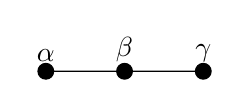
\begin{tikzpicture}
\draw[fill=black] 
(0,0) circle [radius=.1] node [above] {$\alpha$} --
(1,0) circle [radius=.1] node [above] {$\beta$} --
(2,0) circle [radius=.1] node [above] {$\gamma$};
\end{tikzpicture}.
  
For $m\geq 2$ define $G_m$ as the group presented by generators $\mathcal{X}_m$ and the following three families of relations:
\begin{align}
 \label{eq:am} \tag{$a_m$} x_{\alpha}(\xi) x_{\alpha}(\eta) & = x_{\alpha}(\xi+\eta),&  \xi,\eta\in B_d,\ d\leq m;&\\
 \label{eq:bm} \tag{$b_m$} [x_\alpha(\xi), x_{\alpha'}(\eta))] &  = 1, & \text{in the case $\alpha+\alpha'\not\in\Phi\cup\{0\}$,}\\
 \nonumber                                                     &       & \xi \in B_d,\ \eta \in B_e,\ d,e\leq m;\\
 \label{eq:cm} \tag{$c_m$} [x_\alpha(\xi), x_{\alpha'}(\eta)] & = x_{\alpha+\alpha'}(N_{\alpha,\alpha'}\xi\eta), & \text{in the case $\alpha+\alpha'\in \Phi$,}\\
 \nonumber                                                    &  & \xi \in B_d,\ \eta \in B_e,\ d, e, d+e \leq m.
 \end{align}
For $m=1$ define $G_1$ as the group presented by generators $\mathcal{X}_1$, 
three above families of relations $(a_1), (b_1), (c_1)$ and the following additional family:
\begin{align}  \label{eq:d1} \tag{$d_1$} [[x_{\alpha+\beta+\gamma}(\xi), x_{-\gamma}(\eta)], x_{\beta+\gamma}(\zeta) ] & = 1, 
 & \xi,\eta,\zeta\in B_1,\ \text{ $(\alpha, \beta, \gamma)$ is an $\rA_3$-triple. }
\end{align}

The obvious embedding of generators $\mathcal{X}_m \subseteq \mathcal{X}_{m+1}$ induces a map $f_m\colon G_m \to G_{m+1}$.
Our goal is to show the following result.
\begin{prop}\label{prop:tul3.3}
 For $m\geq 1$ the map $f_m$ is an isomorphism. Consequently, $\St(\Phi, B)$ can be presented by generators $\mathcal{X}_1$ and relations $(a_1)$, $(b_1)$, $(c_1)$, $(d_1)$.
\end{prop}
\begin{rem}
   Notice that for $\Phi=\rA_\ell$, $\ell\geq 4$ the group $\St(\Phi, B)$ admits a shorter presentation with family~ $(d_1)$ omitted (see~\cite[Lemma~3.3]{Tu83}).
   This is also true for $\Phi=\rE_\ell$ since $\St(\rE_\ell, R)$ can be presented as an amalgamated product of several copies of $\St(\rA_4, R)$, (cf. e.\,g.~\cite[Lemmas~3,7)]{S15}).   
  On the other hand, we believe that the above presentation is the shortest possible in the cases $\Phi=\rA_3, \rD_\ell$. \end{rem}

We will use the following commutator identities (cf.~\cite[H1]{Re75}):
\begin{align}
 \label{eq:H1ii}  [ab, c] = {}^a[b, c] \cdot [a,c];&\\ %= [a,[b,c]]\cdot [b,c] \cdot [a,c];&\\
 \label{eq:H1iii} [a,c]   = 1    \text{ implies } [a, [b,c]] = [[a,b],{}^bc].&
\end{align}

\begin{lemma}
 Suppose $m \geq 1$.
 Let $\alpha, \beta, \alpha', \beta' \in \Phi$ be such that $\alpha + \beta = \alpha' + \beta'$.
 Assume, moreover, that $\xi \in B_d$, $\xi' \in B_{d'}$, $\eta \in B_e$, $\eta' \in B_{e'}$ are such that 
  $N_{\alpha, \beta} \xi \eta = N_{\alpha', \beta'}\xi' \eta'$ for some $d,d',e,e'\leq m$ satisfying $d+e=d'+e' = m+1$.
 Then the following relations holds in $G_m$:
 \begin{equation}
  \label{eq:S-correctness} [x_\alpha(\xi), x_\beta(\eta)] = [x_{\alpha'}(\xi'), x_{\beta'}(\eta')].
 \end{equation}
 Moreover for every $\zeta \in B_{k''}$, $k''\leq m$ and $\gamma\in\{\alpha, \beta, \alpha + \beta\}$
  the following relation holds in $G_m$:
 \begin{equation}
 \label{eq:S-commutes} [[x_\gamma(\zeta), [x_\alpha(\xi), x_\beta(\eta)]] = 1.
 \end{equation}
\end{lemma}
\begin{proof}
 Notice that $k+l = m+1$, $k, l\leq m$ imply $k,l>0$, hence $B_i= A \cdot t^i$ for $i=k,k',l,'l'$.
 This means that without loss of generality we may assume that $\mathfrak{m}=0$ and $B = A[t]$.
 But now our statement is not different from~\cite[Proposition 1.1]{Re75} (or~\cite[Proposition~3.2.2]{RS76} in the case $g=1$)
  and can be proved by the same argument which remains valid for a general coeffient ring $A$.
\end{proof}

For every $\xi \in B_{m+1}$ and $\alpha\in \Phi$ there exist $\xi' \in B_m$ and $\alpha'\in \Phi$ such that $\xi = t\xi'$ and $\alpha-\alpha'\in\Phi$,
so we can define the following element of $G_m$:
\begin{equation} \label{eq:S-definition} S_\alpha(\xi) := [x_{\alpha-\alpha'}(N_{\alpha-\alpha',\alpha'} \xi'), x_{\alpha'}(t)].\end{equation} 
From~\eqref{eq:S-correctness} it follows that $S_\alpha(\xi)$ does not depend of the choice of $\alpha'$.

Let us show that elements $S_\alpha(\xi)$ satisfy the relations $(a_{m+1})$, $(b_{m+1})$ and $(c_{m+1})$.
From \eqref{eq:H1ii} and~\eqref{eq:S-commutes} it follows that $S_\alpha(\xi)$ satisfy $(a_{m+1})$ and hence $(b_{m+1})$ in the special case $\alpha=\alpha'$.
\begin{lemma} \label{lem:cm-plus1} Suppose that $m\geq 1$. For every $\alpha, \alpha' \in \Phi$ such that $\alpha+\alpha' \in \Phi$ and
 $a\in A$, $\xi \in B_d$, $d \leq 0$ the following relation holds in $G_m$: 
\begin{equation} \nonumber
[x_\alpha(\xi), S_{\alpha'}(at^{m+1})] = [x_\alpha(t\xi), x_{\alpha'}(at^m)] = S_{\alpha+\alpha'}(N_{\alpha,\alpha'}a\xi t^{m+1}).
\end{equation}
\end{lemma}
\begin{proof}
By \cite[Lemma~3.1.2]{RS76} we may assume without loss of generality that $\alpha'=\beta$ for some $\rA_3$-triple $(\alpha, \beta, \gamma)$.
\begin{align*}
   [x_\alpha(\xi), S_\beta(at^{m+1})] = [x_\alpha(\xi), [x_{\beta + \gamma}(t), x_{-\gamma}(a't^m)]]
   &  \text{ by~\eqref{eq:S-correctness},\eqref{eq:S-definition} for $a' = N_{\beta+\gamma, -\gamma} a$} \\ 
 = [x_{\alpha+\beta+\gamma}(\epsilon t\xi), {}^{x_{\beta+\gamma}(t)}x_{-\gamma}(a't^m)]             
 &  \text{ by~\eqref{eq:H1iii}, for $\epsilon=N_{\alpha, \beta+\gamma}$} \\
 = {}^{x_{\beta+\gamma}(t)}[x_{\alpha+\beta+\gamma}(\epsilon t\xi), x_{-\gamma}(a't^m)]             
 &  \text{ by $(b_1)$}
\end{align*} 
Denote by $R$ the expression in the right hand side of the above formula.
\begin{enumerate}
 \item \label{case:cm-1} Case $m=1$, $d = 0$.
 \begin{align*}
   R  = [x_{\alpha +\beta + \gamma}(\epsilon t\xi), x_{-\gamma}(a't)] 
   & \text{ by $(d_1)$}\\
      = {}^{x_{\beta+\gamma}(1)}[x_{\alpha +\beta + \gamma}(\epsilon t\xi), x_{-\gamma}(a't)] 
   & \text{ by~\eqref{eq:H1ii}, $(b_1)$, $(c_1)$} \\
      = [x_\alpha(\xi), [x_{\beta + \gamma}(1), x_{-\gamma}(a't^m)]] 
   & \text{ by $(b_1)$, \eqref{eq:H1iii}}\\
      = [x_\alpha(t\xi), x_\beta(at)]
   & \text{ by~\eqref{eq:S-correctness},\eqref{eq:S-definition}.}
 \end{align*}  
 \item \label{case:cm-2} Case $m\geq 2$ or $m=1$, $d < 0$.
 \begin{align*}
 R = {}^{x_{\beta+\gamma}(t)}[x_{\alpha+\beta+\gamma}(\epsilon t^2\xi), x_{-\gamma}(a't^{m-1})]     
 &  \text{ by~\eqref{eq:S-correctness} if $k=0$ or~\eqref{eq:cm} if $k <0$} \\
 = [[x_\alpha(t\xi), x_{\beta+\gamma}(t)], {}^{x_{\beta+\gamma}(t)} x_{-\gamma}(a't^{m-1})]         
 &  \text{ by~$(b_2)$, $(c_2)$ or by~\eqref{eq:S-commutes},\eqref{eq:S-definition} if $m=1$} \\
 = [x_\alpha(t\xi), x_\beta(at^m)]                                                                  
 &  \text{ by~\eqref{eq:H1iii}. \qedhere}
\end{align*} 

\end{enumerate}
\end{proof}

It will be convenient for us to extend the definition of $S_\alpha(\xi)$ by allowing $\xi$ to take values in $B_d$ for $d\leq m$.
In this case we simply set $S_\alpha(\xi) = x_\alpha(\xi)$.

Now suppose  $0 \leq d \leq m+1$. Clearly \eqref{eq:S-correctness} and \eqref{eq:S-definition} (in the case $1\leq d\leq m$) or~\cref{lem:cm-plus1} (in the case $d=0,m+1$) imply that
\begin{equation} \label{eq:cm-plus1-generalized} 
[S_\alpha(\xi), S_{\alpha'}(\eta)] = S_{\alpha+\alpha'}(N_{\alpha,\alpha'}\xi \eta),\ \xi \in B_d, \eta \in B_{m+1-d}.
\end{equation}

We need to introduce additional notation.
For $a,b\leq m+1$ we denote by $\bot(a, b)$ (resp. $\angle(a,b)$) the family of all relations $[S_\alpha(\xi), S_{\alpha'}(\eta)] = 1$
for which $\xi \in B_a$, $\eta \in B_b$ and $\alpha$ and $\alpha'$ are orthogonal (resp. form a sharp angle). 
We denote by $\bot_0(a, b)$ the subset of $\bot(a, b)$
consisting of those relations for which $\xi = t^{a} \in B_a$.

\begin{lemma} \label{claim1} In $G_m$ relations $\bot_0(1, d)$ and $\angle(d, m)$ imply $\angle(d, m+1)$ for $d\leq m+1$ \end{lemma}
\begin{proof}
Without loss of generality we may assume that $\alpha' = \alpha + \beta$
  for some $\rA_3$-triple $(\alpha, \beta, \gamma)$.
Write $\eta = bt^{m+1}$ for some $b\in A$.
\begin{align*} 
[S_\alpha(\xi), S_{\alpha+\beta}(bt^{m+1})] = [S_\alpha(\xi), [x_{\alpha+\beta+\gamma}(b't^m), x_{-\gamma}(t)]] & \text{ by~\eqref{eq:S-correctness} and~\eqref{eq:S-definition}}\\
= [[S_\alpha(\xi), x_{\alpha+\beta+\gamma}(b't^m)], {}^{x_{\alpha+\beta+\gamma}(b't^m)}\!x_{-\gamma}(t)] & \text{ by~$\bot_0(1, d)$}\\
= 1
 & \text{ by~$\angle(d, m)$. \qedhere} \end{align*} 
\end{proof}

\begin{lemma} \label{claim2} In $G_m$ relations $\angle(d, m+1)$ imply $\bot_0(d, m+1)$ for  $1\leq d\leq m+1$. \end{lemma}
\begin{proof}
As before, without loss of generality we may assume $\alpha' = \gamma$ for some $\mathsf{A}_3$-triple $(\alpha, \beta, \gamma)$.
 \begin{align*}
 {}^{S_\gamma(t^d)}S_\alpha(bt^{m+1}) = {}^{S_\gamma(t^d)}[S_{-\beta}(b't^{m+1}), x_{\alpha+\beta}(1)] & \text{ by~\cref{lem:cm-plus1}}\\
 = [S_{-\beta}(b't^{m+1}), {}^{S_\gamma(t^d)}x_{\alpha+\beta}(1)]                                     
 & \text{ by $\angle(d, m+1)$}\\
 = [[x_{-\beta-\gamma}(b''t^{m+1-d}), S_\gamma(t^d)], {}^{S_\gamma(t^d)}x_{\alpha+\beta}(1)]          
 & \text{ by~\eqref{eq:cm-plus1-generalized}}\\
 = [x_{-\beta-\gamma}(b''t^{m+1-d)}), [S_\gamma(t^d), x_{\alpha+\beta}(1)]]                           
 & \text{ by~\eqref{eq:H1iii} and $(b_{m+1-d})$}\\
 = S_{\alpha}(b'''t^{m+1})                                                                            
 & \text{ by~\eqref{eq:cm-plus1-generalized}.} \end{align*}
Usual identities for structure constants imply (cf.~\cite[p.~12]{Re75}):
 $b'''=N_{-\beta-\gamma, \alpha+\beta+\gamma} \cdot N_{\gamma, \alpha+\beta} \cdot N_{-\beta-\gamma, \gamma} \cdot N_{-\beta, \alpha+\beta} \cdot b = b,$ from which the claim follows.
\end{proof}

\begin{lemma} \label{claim3}
 In $G_m$ relations $\bot_0(d, m+1)$, $\angle(d, d)$ and $\angle(m+1, m+1)$ imply $\bot(d, m+1)$ for $d\leq m+1$.
\end{lemma}
\begin{proof}
 \begin{align*} 
 S_{\alpha+\beta+\gamma}(abt^{m+1}) = {}^{S_{-\beta}(t^d)}\!S_{\alpha+\beta+\gamma}(abt^{m+1}) 
 & \text{ by $\bot_0(d, m+1)$}\\
 = {}^{S_{-\beta}(t^d)}\![x_{\alpha+\beta}(b't^{m+1-d}), S_\gamma(at^d)] 
 & \text{ by~\eqref{eq:cm-plus1-generalized}} \\
 = [S_{\alpha}(b't^{m+1}) x_{\alpha+\beta}(b't^{m+1-d}), S_\gamma(at^d)] 
 & \text{ by~\eqref{eq:cm-plus1-generalized} and $\angle(d, d)$ }\\
 = {}^{S_{\alpha}(b't^{m+1})}\!S_{\alpha+\beta+\gamma}(abt^{m+1}) [S_{\alpha}(b't^{m+1}), S_\gamma(at^d)] 
 & \text{ by~\eqref{eq:H1ii} and~\eqref{eq:cm-plus1-generalized}} \\
 = S_{\alpha+\beta+\gamma}(abt^{m+1}) [S_{\alpha}(b't^{m+1}), S_\gamma(at^d)] 
 & \text{ by $\angle(m+1, m+1)$. \qedhere}
\end{align*}
\end{proof}

\begin{lemma} \label{lem:bm-plus1}
Elements $S_\alpha(\xi)$ satisfy relations $(b_{m+1})$.
 \end{lemma}
\begin{proof}
We must show that $S_\alpha(\xi)$ satisfy $\angle(d, m+1)$ and $\bot(d, m+1)$ for $d\leq m+1$.
\begin{enumerate}
 \item Relations $\angle(d, m+1)$, $d\leq m$ follow from~\cref{claim1}. 
 \item Relations $\bot(d, m+1)$ with $d\leq 0$ can verified by direct computation:
 \begin{align*} 
 [x_\alpha(\xi), S_{\gamma}(bt^{m+1})] = [x_\alpha(\xi), [x_{\beta+\gamma}(b't^m), x_{-\beta}(t)]] & \text{ by~\eqref{eq:S-correctness},\eqref{eq:S-definition}} \\
 = [[x_\alpha(\xi), x_{\beta+\gamma}(b't^m)], {}^{x_{\beta+\gamma}(b't^m)}\!x_{-\beta}(t)] &
 \text{ by \eqref{eq:H1iii} and $(b_1)$} \\
 = {}^{x_{\beta+\gamma}(b't^m)}\![x_{\alpha+\beta+\gamma}(b't^m\xi), x_{-\beta}(t)] &
 \text{ by $(b_m)$ and $(c_m)$} \\
 = 1 & \text{ by $(b_m)$.}
\end{align*}
 \item Relations $\bot_0(d, m+1)$ with $1\leq d\leq m$ follow from~\cref{claim2}.
 \item Relations $\angle(m+1, m+1)$ follow from~\cref{claim1}, consequently relations $\bot_0(m+1, m+1)$ follow from~\cref{claim2}.
 \item Relations $\bot(d, m+1)$, $0\leq d\leq m+1$ follow from~\cref{claim3} and the previous two assertions.
\end{enumerate}
\end{proof}

\begin{proof}[Proof of~\cref{prop:tul3.3}]
Define the map $g_m\colon G_{m+1} \to G_m$ by $g_m(x_\alpha(\xi)) = S_\alpha(\xi)$.
In view of the above lemmata this map is well-defined. It is clear that $g_m$ is inverse to $f_m$, which proves the first claim.

Denote by $G_\infty$ the group presented by generators $\mathcal{X}_\infty$ and relations $(a_\infty)$, $(b_\infty)$, $(c_\infty)$.
By the above argument there is an isomorphism between $G_1$ and $\colim\limits_{n\to\infty} G_n \cong G_\infty$.

Denote by $i\colon G_\infty \to \St(\Phi, B)$ the map induced by the obvious embedding of $\mathcal{X}_\infty$ into the set of 
 Steinberg generators of $\St(\Phi, B)$.  
Using~\eqref{eq:H1ii} multiple times it is not hard to show that the map $j\colon \St(\Phi, B) \to G_\infty$ given by
 $j(x_\alpha(b)) = \prod x_\alpha(b_i)$, where $b = \sum b_k$ is the decomposition of $b$ into a finite sum of its homogeneous components $b_k\in B_k$, is a well-defined map.
It is clear that $i$ and $j$ are mutually inverse. 
\end{proof}



\section{Overview of Tulenbayev's proof of $K_2$-analogue of Serre problem}

\begin{lemma} \label{lem:3.1f} Let $A$ be a local ring then any element $\alpha \in \St(\Phi, A)$ can be presented as a product 
$ $
 
\end{lemma}


\section{Proof of the main result}

\subsection{$\sigma$-pairs}
Notice that for $\varpi \in P(\Phi^\vee)$ and $\beta \in \ZZ \Phi$ one has $(\varpi, \beta) \in \ZZ $.
Consequently, for $\varepsilon \in R^*$ and $\varpi \in P(\Phi^\vee)$ the formula $\chi_{\varpi, \varepsilon}(\beta) = \varepsilon ^ {(\varpi, \beta)}$
defines a character $\chi_{\varpi, \varepsilon} \in \Hom(\ZZ \Phi, R^*)$.

Consider the action of $H=\Hom(\ZZ \Phi, R^*)$ on the set of generators $\mathcal{X}_{\Phi, R}$ of the Steinberg group $\St(\Phi, R)$ given by
\begin{equation} \chi \cdot x_\alpha(\xi) = x_\alpha(\chi(\alpha) \cdot \xi),\ \chi \in H,\ \alpha\in \Phi,\ \xi \in R. \end{equation}
Since $\chi$ is a character, this action respects the set of Steinberg relations $\mathcal{R}_{\Phi, R}$ and therefore gives a well-defined action of $H$ on $\St(\Phi, R)$.

In the sequel we will be mostly interested in the following example.
\begin{example}
Let $A$ be a ring, denote by $R$ the ring $A[t, t^{-1}]$ of Laurent polynomials over $A$ and let $\alpha_i \in \Pi$ be a simple root.
Define automorphisms $\beta_i^+$ and $\beta_i^-$ of $\St(\Phi, R)$ via $\beta_i^+ = \chi_{\varpi_i, t}$, $\beta_i^- = \chi_{\varpi_i, t^{-1}}$.
It is easy to see that
\begin{equation}\label{eq:sigma_act} \beta_i^\pm(x_\alpha(\xi)) = x_\alpha(t^{\pm m_i(\alpha)} \cdot \xi).\end{equation}
\end{example}

One of the key steps of in the proof of Suslin lemma for $K_2$ is to define analogue of maps $\beta_i^\pm$ on the level of the group $\St(\Phi, A[t])$.
Of course, one cannot expect such maps to be automorphisms or even be defined on the whole group $\St(\Phi, A[t])$.
Thus, our first goal is to define the subgroups of $\St(\Phi, A[t])$ on which these morphisms could, in principle, be defined.

In the sequel we assume that $i$ is a vertex of the Dynkin diagram $D(\Phi)$ of $\Phi$ with the property that $m_i(\alpha_{\max})=1$ (of course, this implies that $\Phi$ is not of type $\rE_8, \rF_4$ or $\rG_2$).
Denote by $\mathcal{X}_i$ (resp. $\mathcal{X}^i$) the subsets of $\mathcal{X}_{\Phi, A[t]}$ consisting of those generators $x_{\alpha}(\xi)$ of $\St(\Phi, A[t])$ for which 
$m_i(\alpha) > 0$ (resp. $m_i(\alpha)<0$) implies that $\xi \in A[t]$ is divisible by $t$.
% either $i\neq k$ (resp. $j\neq k$) or $\xi\in R[t]$ is divisible by $t$.
Denote by $N_i$ and $N^i$ the subgroups of $\St(\Phi, A[t])$ generated by $\mathcal{X}_i$ and $\mathcal{X}^i$, respectively.
%Our goal is to construct mutually inverse morphisms $\sigma_k$, $\sigma_k^{-1}$ fitting into the following diagram.

\begin{dfn} A pair of mutually inverse maps $(\sigma_i^+, \sigma_i^-)$ between the groups $N^i$ and $N_i$ will be called a {\it $\sigma$-pair corresponding to the vertex $i\in D(\Phi)$},
 if these maps fit into the following diagram.
\begin{equation} \label{eq:sigma-diagram}
\xymatrix{ N_i\ar@{-->}[r]^{\sigma_i^+}\ar[d] & N^i \ar[d] \ar@{-->}[r]^{\sigma_i^-} & N_i \ar[d] \\ 
          \St(\Phi, R) \ar@<-0.0ex>[r]_{\beta_i^+} & \St(\Phi, R) \ar@<-0.0ex>[r]_{\beta_i^-} & \St(\Phi, R)} 
\end{equation}
In the above diagram the vertical arrows are canonical embeddings of $N_k$ and $N^k$ into $\St(\Phi, A[t])$ postcomposed with 
 the map of Steinberg groups induced by the embedding $A[t] \hookrightarrow R = A[t, t^{-1}]$.
%As before, we denote by $R$ the ring $A[t, t^{-1}]$ of Laurent polynomials over $A$.
         % \GL(n, R) \ar@<-0.0ex>[r]_{(-)^{\delta_k}} & \GL(n, R) \ar@<-0.0ex>[r]_{{}^{\delta_k}(-)} & \GL(n, R)
\end{dfn}

For the remainder of this subsection our main goal will be to verify that an analogue of the group decomposition from \cite[Lemma~3.1f]{Tu83} holds for $\St(\Phi, A)$
 provided $\St(\Phi, R)$ admits at least one $\sigma$-pair.

Denote by $\widetilde{W}$ the subgroup of $\St(\Phi, A)$ generated by elements $w_\alpha(1)$.
The subgroup $\widetilde{W}$ acts on $\St(\Phi, A)$ via conjugation, for example, 
 the action on the generators of $\mathcal{X}_{\Phi, A}$ can be expressed via the formula ${}^{w_\alpha(1)} \!x_{\beta}(\xi) = x_{\sigma_{\alpha}(\beta)} ( \pm \xi)$.
It is easy to see that the action of $\widetilde{W}$ on the set of root subgroups $\{X_\alpha \mid \alpha \in \Phi \}$ of $\St(\Phi, R)$ coincides with the obvious
 action of the Weyl group $W(\Phi)$ on it. Since $N_i$ and $N^i$ are generated by root subgroups we immediately obtain the following statement.
\begin{lemma} The set of elements in the orbit of $N_i$ (resp. $N^i$) under the conjugation action of $\widetilde{W}$ 
is in bijective correspondence with 
the set of adjacency classes of $W(\Phi)$ with respect to its Levi subgroup $W_i = W(\Delta_i)$. %TODO: Unsure whether it is true at all :)
\end{lemma}
In the sequel we denote by $\Sigma$ the set of elements in $\widetilde{W}$ whose projections in $W(\Phi)$ form the set of representatives for
 right adjacency classes of $W(\Phi)$ with respect to $W_i$. %We can assume these representatives to be short


\subsection{Structure theorem for Steinberg groups}


sufficient conditions implying the main structure result for Steinberg groups.

Let $\mu$ be a microweight of the root system $\Phi$. Denote by $N_\mu$

\subsection{Construction of \texorpdfstring{$\sigma$}{sigma}-morphisms for $\SL_4$}
Let $R$ be a local ring and assume that $n\geq 4$.
For $1\leq k\leq n$ denote by $\delta_k$ the $n\times n$ matrix of $\GL(n, R[t, t^{-1}])$ which differs from the unit matrix 
 only by the element $t$ on the $k$-th place of its diagonal.
Recall from~\cite[Corollary~4]{Ka77} that there exists unique automorphisms $\beta_{\delta_k}$, $\beta_{\delta_k^{-1}}$ of $\St(n, R[t, t^{-1}])$
 modeling conjugation with matrices $\delta_k$ and $\delta_k^{-1}$ (see diagram~\eqref{eq:sigma-diagram} below)

For $n\geq 5$ $\sigma-$morphisms have already been constructed by Tulenbaev, see \S~3 of~\cite{Tu83}.
Thus, in the sequel we are mainly interested in the case $n=4$.
To simplify notation, we limit ourselves to constructing the map $\sigma_1$, so everywhere in the sequel we assume that $k=1$. 

Of course, the map of right conjugation with $\delta_1$ induces the obvious one-to-one set-theoretic correspondence between $\mathcal{X}_1$ and $\mathcal{X}^1$. 
However, there seems to be no reasonable description of the complete set of relations between the elements $\mathcal{X}_1$ that would allow one to describe $N_1$
 as a group given by generators and relations.
Thus, in order to define $\sigma_1$ we will use the alternate description of $N^1$ given in terms of ``another presentation''.
We start with the following simple observation.
\begin{lemma} \label{lem:n1-decomp} There is an isomorphism $N_1 \cong N_{1,0} \rtimes P_1^-(R)$, where $N_{1,0}$ denotes the subgroup $\St(n, R[t], tR[t])$
 and $P_1^-(R)$ is the subgroup of $\St(n, R)$ generated by $x_{ij}(\xi)$ with $i\neq 1$.
\end{lemma}

Recall that the universal property of semidirect products asserts that for any group $H$ acting on a group $N$ via $\phi \colon H \to \Aut(N)$ and any group homomorphisms
 $f_N\colon N \to G$, $f_H\colon H \to G$ satisfying 
\begin{equation} \label{eq:coherence-condition} f_N(\phi(h)(n)) = f_H(h) f_N(n) f_H(h)^{-1},\ n\in N,\ h\in H,\end{equation} there exists a unique map $f\colon N \rtimes H \to G$
 extending $f_N$ and $f_H$. 
Thus, by the above lemma, in order to construct the map $\sigma_1$ we need to construct the following two maps and verify that they satisfy~\eqref{eq:coherence-condition}:
\[ (\sigma_1)_{P_1^-(R)} \colon P_1^-(R) \to N^1, \ \ (\sigma_1)_{N_{1,0}} \colon N_{1,0} \to N^1.\]

It is easy to define the first map $(\sigma_1)_{P_1^-(R)}$.
Using the decomposition $P_1^-(R) \cong U^-_1 \rtimes L_1$ where 
\[U^-_1 = \langle x_{i1}(\xi) \mid i\neq 1,\ \xi\in R \rangle \text{ and } L_1 = \langle x_{ij}(\xi) \mid i,  j \neq 1,\ \xi\in R\rangle \]
we apply the universal property of semidirect products once again 
 and define $(\sigma_1)_{P_1^-(R)}$ by requiring that it acts identically on $L_1$ 
and acts on elements of $U^-_1$ via the formula $(\sigma_1)_{P_1^-(R)}(x_{i1}(\xi))= x_{i1}(t\xi)$.

Before we proceed with the construction of the second map $(\sigma_1)_{N_{1,0}}$ we need to recall several technical
 constructions pertaining to ``another presentation'' of the group $N_{1,0}$.

For $u \in R^n$ we denote by $D(u)$ the subset of $R^n$ consisting of all $v$ satisfying $u^tv = 0$ and having at least two zero entries.
Recall from 3.2 of~\cite{Ka77} that for every $u, v, w \in R[t]^n$ such that $u^t \cdot v = 0$ there
 is a decomposition of $(w^t u) \cdot v$ into a sum of elements of $D(u)$, called {\it canonical decomposition}:
\setcounter{equation}{1}
\renewcommand{\theequation}{\arabic{equation}}
\begin{equation} \label{eq:canonical} (w^tu) \cdot v=\sum_{i<j}u_{ij} c_{ij}(v, w),\end{equation}
where $u_{ij}=e_iu_j-e_ju_i,$ and $c_{ij}(v, w)=v_iw_j-v_jw_i.$

Let $A$ be a commutative ring and $I$ be a splitting ideal of $A$.
Let $u, v \in A^n$ be such that $u^t v = 0$ and assume, moreover, that either $u$ or $v$ has at least one zero entry.
Recall from 3.8, 3.10 of~\cite{Ka77} that under these assumptions one can define certain element
 $x(u, v)$ of $\St(n, A)$ such that $\pi(x(u, v)) = t(u, v) = 1 + uv^t$.
The following properties of $x(u, v)$ are standard (cf.~\cite[Lemma~1.1]{Tu83}).
\begin{lemma} \label{lem:xsmall-properties}
\begin{lemlist}
 \item \label{item:xsmall-scalar} If $v$ or $w$ has at least two zero components, then 
 \begin{equation}\nonumber x(v, wa) = x(va, w).\end{equation}
 \item \label{item:xsmall-additivity} If $w_1$ and $w_2$ have at least one common zero coordinate then
 \begin{equation}\nonumber x(v, w_1)x(v, w_2) = x(v, w_1+w_2).\end{equation}
 \item \label{item:xsmall-commute} If $v$, $v'$ are simultaneously orthogonal to $w$ and $w'$ and the elements $w, w'$
  both have at least two zero components then $x(v, w)$ and $x(v', w')$ commute.
\end{lemlist}
\end{lemma}

Let $u \in E(n, A)e_1$, $v \in I^n$ be such that $u^tv = 0$.
Recall from \S~4 of~\cite{LS17} that one can define the following elements of $\St(n, A, I)$:
\begin{equation} \label{eq:sigma-definition}
 F(u, v) = \prod\limits_{i=1}^r x(u,  v_i),\ \
 S(v, u) = \prod\limits_{i=1}^r x( v_i, u).
\end{equation}
Here $\{v_r\}$, $r=1,\ldots,N$ is any collection of elements of $I^n \cap D(u)$ such that $\sum_{r=1}^N v_r = v$.
Since $u$ is unimodular, such a collection always exists by~\eqref{eq:canonical}, moreover
 $F(u, v)$ and $S(u, v)$ do not depend on its choice. %TODO: Give reference

Recall from~\cite{LS17} that it is possible to give a presentation of the relative Steinberg group $\St(n, A, I)$ formulated in terms of elements $F(u, v)$, $S(v, u)$.
More formally, \cite[Proposition 3.10]{LS17} asserts that $\St(n,\,A,\,I)$ admits presentation with the set of generators
\begin{multline*} \{F(u,\,v)\mid u\in E(n,\,A)e_1,\ v\in I^n,\ u^tv=0\}\, \cup \\ \cup \{S(u,\,v)\mid u\in I^n,\ v\in E(n,\,A)e_1,\ u^tv=0\}\end{multline*}
subject to relations
\setcounter{equation}{0}
\renewcommand{\theequation}{R\arabic{equation}}

\begin{align}
&F(u,\,v)F(u,\,w)=F(u,\,v+w), \label{add4}\\
&S(u,\,v)S(w,\,v)=S(u+w,\,v), \label{add5}\\
&F(u,\,v)F(u',\,v')F(u,\,v)^{-1}=F(t(u,\,v)u',\,t(v,\,u)^{-1} v'), \label{conj3} \\
&F(ge_1,\,g^*e_2a)=S(ge_1a,\,g^*e_2),\ \text{for all}\ a\in I,\, g \in E(n, A).
\end{align}
Here $g^*$ denotes the contragradient matrix, i.\,e. $g^* = {g^{-1}}^t$ and $e_i$ is the standard basis vector of $A^n$.

\setcounter{equation}{3}
\renewcommand{\theequation}{\arabic{equation}}

To define the map $(\sigma_1)_{N_{1,0}}$ we will invoke the above presentation in the special case $A=R[t]$, $I=tR[t]$.
Indeed, define $\sigma_1$ on $N_{1,0}=\St(n, R[t], tR[t])$ by the following identities: 
\begin{equation}
 \sigma_1(F(u, v)) = \prod\limits_{i=1}^r x(\delta_1^{-1} \cdot t u, \delta_1 \cdot t^{-1} v_i),\ \
 \sigma_1(S(v, u)) = \prod\limits_{i=1}^r x(\delta_1^{-1} \cdot v_i, \delta_1 \cdot u).
\end{equation}

\begin{lemma} \label{lem:cor-conj}
 \begin{lemlist}
   \item \label{item:correctness} The elements $\sigma_1(F(u, v))$ and $\sigma_1(S(v, u))$ are well-defined, i.\,e. they do not depend on the choice of decomposition for $v$.
   \item \label{item:conjugation} For any $g \in N^1$ one has 
      \begin{equation}
          \nonumber {}^g\left(\sigma_1(F(u, v))\right) = \sigma_1\left(F(g' \cdot u, {g'}^{*} \cdot v)\right),\ \ 
                    {}^g\left(\sigma_1(S(u, v))\right) = \sigma_1\left(S(g' \cdot u, {g'}^{*} \cdot v)\right),                    
      \end{equation}
      where $g' = {}^{\delta_1}\pi(g).$
 \end{lemlist}
\end{lemma}
\begin{proof}[Short proof]
 The first assertion can be easily verified using the canonical decomposition and~\cref{lem:xsmall-properties}
  (compare with Tulenbaev's argument after~\cite[Lemma~1.1]{Tu83}).
  
 The second assertion can be proved similarly to~\cite[3.14]{Ka77}, (cf. also with the proof of~\cite[Lemma~4.4d]{LS17}).
\end{proof}
\begin{proof}[Long proof]
 Let us verify the first assertion. Let $v = \sum_r v^r$ be a decomposition as above. 
 Since each $v^r$ is orthogonal to $u$ we can write the canonical decomposition  
 $v^r = \sum_{i<j} u_{ij} c_{ij}(v^r, w)$, moreover, $\sum_{r} c_{ij}(v^r, w) = c_{ij}(v, w)$.
 \cref{lem:xsmall-properties} allows us to rewrite the right-hand side of~\ref{eq:sigma-definition} in such a way that 
  it does not depend on the choice of decomposition for $v$:
 \begin{multline}
  \prod\limits_r x(\delta_1^{-1} ut, \delta_1 v^rt^{-1}) = \prod\limits_{r}\prod\limits_{i<j} x(\delta_1^{-1} ut, \delta_1 u_{ij}c_{ij}(v^r, w)t^{-1}) = \\ 
   = \prod\limits_{i<j} x(\delta_1^{-1} ut, \delta_1 u_{ij}c_{ij}(v, w)t^{-1}). 
 \end{multline}

 We only verify the second assertion for $F(u, v)$  and only in the special case $g = x_{hk}(\xi) \in \mathcal{X}^1$, $g' = t_{hk}(\xi') \in \pi(\mathcal{X}_1)$.
 Choose $w\in R^n$ so that $w^t u = 1$ and write $v = \sum_{1\leq i<j\leq n} u_{ij} c_{ij}$, where $u_{ij}$ and $c_{ij} = c_{ij}(v, w)$ are as in~\eqref{eq:canonical}. 
 We can write ${}^g\left(\sigma_1\left(F(u, v)\right)\right)$ as follows:
 \begin{equation} \nonumber
   \prod\limits_{1\leq i<j\leq n} x(\pi(g) \cdot \delta_1^{-1} \cdot t u, \pi(g)^* \cdot \delta_1 \cdot t^{-1} u_{ij}c_{ij})
                                   = \prod\limits_{1\leq i<j\leq n} x(\delta_1^{-1} \cdot g'\cdot t u, \delta_1 \cdot {g'}^* \cdot t^{-1} u_{ij}c_{ij}).
 \end{equation} 
 Now for every factor in the right-hand side we do the following.
 If $\{i, j\} = \{h, k\}$ or $\{i, j\} \cap \{h, k\} = \emptyset$ we leave the term unchanged.
 Otherwise, if, $|\{i, j\} \cap \{h, k\}| = 1$,  say $j = h$, $i\neq k$, we further decompose it as follows:
  \begin{equation} \nonumber
    x(\delta_1^{-1} \cdot t u', \delta_1 \cdot {g'}^* \cdot u_{ij} (c_{ij} t^{-1})) = 
     x(\delta_1^{-1} \cdot u' t, \delta_1 \cdot u'_{ij} (c_{ij} t^{-1})) \cdot 
     x(\delta_1^{-1} \cdot u' t, \delta_1 \cdot u'_{ki} (c_{ij} t^{-1})).
  \end{equation}
  Here $u' = g'  u = t_{jk}(\xi') \cdot u$.
  Notice that ${g'}^*u_{ij} = t_{kj}(-\xi') \cdot u_{ij} = e_iu_j - e_ju_i + e_k\xi'u_i =u'_{ij}+u'_{ki}\xi'$. 
  
  Thus, we arrive at a product $\prod_{s} x(\delta_1^{-1} \cdot u't, \delta_1 \cdot v'_s t^{-1}) $, where $v'_s \in D(u')$ and
   $\sum v'_s = {g'}^*v$. Clearly, this product equals $\sigma_1\left(F(g' \cdot u, {g'}^{*} \cdot v)\right)$ by definition.
\end{proof}

\begin{cor}
 The map $\sigma_1$ preserves relations~\eqref{add4}--\eqref{conj3}.
\end{cor}
\begin{proof}
 For~\eqref{add4}--\eqref{add5} this is an immediate corollary of the first assertion of the previous lemma.
 For~\eqref{conj3} this follows from the second part of the lemma applied in the special case $g = \sigma_1(F(u, v)) \in N^1$.
\end{proof}

It remains to verify that $\sigma_1$ preserves~\eqref{coinc}.
Let us do this at first in the special case when $g^*$ belongs to the subset $G_0 = H_{12}(R) \cdot U^+_1(R) \cdot U^-_1(R)$.
Here we denote by $H_{12}(R)$ the subgroup of $T(n, R)$ generated by semisimple root elements $ h_{12}(\xi)$, $\xi \in R^*$.

Since the only nonzero components of $u = g^* \cdot e_2$ are $u_1$ and $u_2$ we can present $v = g \cdot e_1$ as a sum $v' + v''$, where 
 $v'_i=0$, $i>2$ and $v''_1=v''_2=0$.
Since $v', v'' \in D(u)$ and $u \in D(v)$, from the definition of $\sigma_1$ we obtain that:
\begin{multline} \label{eq:special-case}
 \sigma_1(S(g \cdot e_1a, g^* \cdot e_2)) = x(\delta_1^{-1} \cdot v'a, \delta_1\cdot  u) \cdot x(\delta_1^{-1}\cdot v''a, \delta_1 \cdot u) = \\
  = x(\delta_1^{-1} va, \delta_1 \cdot u) = x(\delta_1^{-1} vat^{-1}, \delta_1 \cdot ut) = \sigma_1(F(g \cdot e_1, g^* \cdot e_2a)) 
\end{multline}

To obtain the assertion in the general case notice that for $R$ local the group $\E(n, R)$ admits the following decomposition:
\[\E(n, R) = \mathrm{EP}_1(R) \cdot H_{12}(R) \cdot U^-_1(R) \cdot U^+_1(R).\]
This can be either obtained as a corollary of Gauss decomposition or can be proved by a direct calculation. %TODO: Give reference

Applying transpose-inverse automorphism $(-)^*$ to the above decomposition and invoking~\cref{lem:n1-decomp} we obtain that $\E(n, R[t]) = \pi(N_1) \cdot G_0$.
Thus, every $g \in \E(n, R[t])$ can be factored as $\pi(n) \cdot h$ for some $n\in N_1$ and $h \in G_0$.
Since $\pi(n) = {}^{\delta_1} \pi(n')$ for some $n' \in N^1$ it remains to apply~\cref{item:conjugation} and~\eqref{eq:special-case} to obtain the required assertion:
\begin{multline} \nonumber \sigma_1(F(g \cdot e_1, g^* \cdot e_2a)) = {}^{n'}(\sigma_1(F(h \cdot e_1, h^* \cdot e_2a))) = \\
                           = {}^{n'}(\sigma_1(S(h \cdot e_1a, h^* \cdot e_2))) = \sigma_1(S(g \cdot e_1a, g^* \cdot e_2)). \end{multline}

Thus, we have completed the construction of the map $(\sigma_1)_{N_{1,0}}$.
It is not hard to verify that the condition~\eqref{eq:coherence-condition} is satisfied with these definitions,
 therefore, we have also completed the construction of the map $\sigma_1$.

\subsection{Proof of the theorem on \texorpdfstring{$\mathbb{P}^1$}{P1}-glueing for $K_2$}

\section{Applications}

\subsection{Bruhat--Tits buildings}

\subsection{\texorpdfstring{$A^1$}{A1}-invariance of the fundamental group}

\DeclareRobustCommand{\VAN}[2]{#2}
\printbibliography

\end{document}
